% !Mode:: "TeX:UTF-8" 

\BiChapter{相关工作综述}{Related Works}
\label{sec:pdpintro}

% \BiSection{本章引论}{Introduction to Chapter}\label{chap21}

\BiSection{网络资源优化}{Network Resource Optimization} \label{chap24}



\BiSubsection{软件定义网络安全通道机制的瓶颈}{The Secure Channel in Software-Defined Network}







\BiSubsection{数据平面流表资源匮乏的问题}{Data Plane Flow Table Resources and Problems}\label{chap242}
%ip1w 2.2.1


1)SDN数据平面查找模型
%key是什么,怎么与ACTION联系



2)各类包头域查找匹配方法











\BiSection{可编程网络的灵活性与性能的矛盾}{Network Programmability}\label{chap22}
%研究领域发展趋势介绍





%\BiSubsection{软件实现---早期网络基础设施}{Software Iimplementation---Early Network Infrastructure} \label{chap221}



%\BiSubsection{软件定义网络演进---软、硬件物理隔离}{Software-Defined Network Evolution--- Physical Isolation}\label{chap223} 

\BiSubsection{软件定义网络的控制接口统一化}{Software-Defined Network Evolution--- Physical Isolation}




\BiSubsection{基于ASIC的可编程网络灵活性有限}{The future of programmable data plane}




%可编程解析器须实现灵活可运行时配置的协议图。可编程解析器中的状态转移图可以通过状态查找表来实现。状态查找表可以由RAM 和/或 TCAM存储器组成,RAM是一种基于地址的内容访问存储器;CAM是一种基于内容的地址访问存储器。CAM中在不同地址存储有内容,当CAM接收到一个内容输入请求(key)时,可以并行搜索所有位置,并返回内容等于key的地址位置。TCAM则是在请求key中可以定义“不考虑”bit位,在判断二者内容是否相等时所有“不考虑”位都认为是相等的。如图\ref{fig:progparser}所示,TCAM的key的宽度与一个完整的包头相等,在TCAM的一个表项中,存储着某一个协议的包头标识数据,这个数据的位置与真实数据包包头中此协议的位置相同,但是其他位置都属于“不考虑”bit位。因而只要包头可以匹配此TCAM表项,就代表包头中有这个协议。当然由于包头域是一种有向图,在不同阶段所需要看的标识位置是不一样的。下一跳状态信息就存储在RAM中,得到新的状态后,电路再去查找TCAM,直到有向图走完。只要我们有足够宽的TCAM表,我们可以通过任意修改表中存储的状态图信息来实现运行时可编程的包头解析器。

%\begin{figure}[htbp]
%	\centering 
%	\vspace{-1.5mm}
%	\begin{minipage}[t]{0.48\textwidth}
%		\centering
%		
\includegraphics[scale=0.9]{traditionalmatch.pdf}
%		\caption{传统交换机中的查找匹配过程} \label{fig:traditionalmatch}
%	\end{minipage}
%	\begin{minipage}[t]{0.48\textwidth}
%		\centering
%		
\includegraphics[scale=0.90]{progmatch.pdf}%此图有更新 2020年7月4日15:28:26
%		\caption{基于ASIC的可编程匹配模型} \label{fig:progmatch}
%	\end{minipage}
%\end{figure}

%第二,需要解决基于ASIC的可编程流表匹配。在传统交换机中,当数据包完成包头域的解析,交换机通过查询流表来得到数据包的执行指令。如图\ref{fig:traditionalmatch}所示,处理每个协议的节点组成了协议有向图,节点一般可以抽象为“匹配--执行”的模式。由于包头协议状态转移图是固化的,所以交换机可操作的数据包的种类、数量也是固定的,其他数据包会被交换机当做未知类型而丢弃。在设计交换机之初,就需要根据各个协议字段不同位宽,不同流表匹配方法,制定固定深度的流表。因而目前固化交换机的数据处理核心都会设计异常复杂,需要适配各种有可能的协议,然而在某一个应用场景中只会存在其中一部分数据包类型,导致了很大能耗和经济的开销。
%
%
%
%
%
%可编程流表须实现灵活配置“查找--执行”逻辑结构。如图\ref{fig:progmatch}所示,目前的设计思路,可编程匹配流水线由$N$个“物理块”(Phy\_Stage)串联而成,每个Phy\_Stage可以独立配置查找表的位宽、深度和类型。而且在每个Phy\_Stage中堆叠了所有类型的“执行器”(Action)模块,在运行时这些部件依次按流水线背靠背方式处理。选路器可以由多路复用器(MUX)或交叉开关(Cross\_Bar)组成。由于这些机构都可以被后期在线配置,在这样的流水线中一个1024bits的并行包头数据进入物理块后由第一个选路器(MUX)选出“待匹配域”送入所需的存储器接口,匹配之后的结果和包头域信息被第二个选路器(Cross\_Bar)送往所需的执行器中进行操作。最后执行器将新的域插入(修改/删除)包头内形成新包头。多个“物理块”可以先后呼应形成一个更复杂的“逻辑块”,最终通过运行时配置这些“物理块”可表达任意类型的协议有向图。

%由于硬件可编程技术的加持,外加比虚拟机更轻量级的容器、高速分布式存储、无服务架构、AI对I/O响应速度的要求,使得网络体系架构设计发展繁荣、爆炸增加。相信在未来业界将会出现更多的应用场景,这些场景也将会不断催生出功能更强大的可编程网络、以及更强大的性能。



\BiSubsection{可编程数据平面的应用与问题}{Application and Problems of Programmable Data Plane}\label{chap233}






\BiSection{网络可编程抽象的分析}{"Turing Completeness" of Network Programmability}\label{chap23}
%完备性与硬件平台的设计思路息息相关。https://www.zhihu.com/question/20115374 知乎问题解答




\BiSubsection{网络编程灵活性}{Common Programmability and Programmable NIC}




%2)可编程抽象

%\BiSubsection{通用可编程性和可编程网卡}{Common Programmability and Programmable NIC}\label{chap231}



%\begin{figure}[!ht]
%	\centering 
%	\vspace{-1.5mm}
%	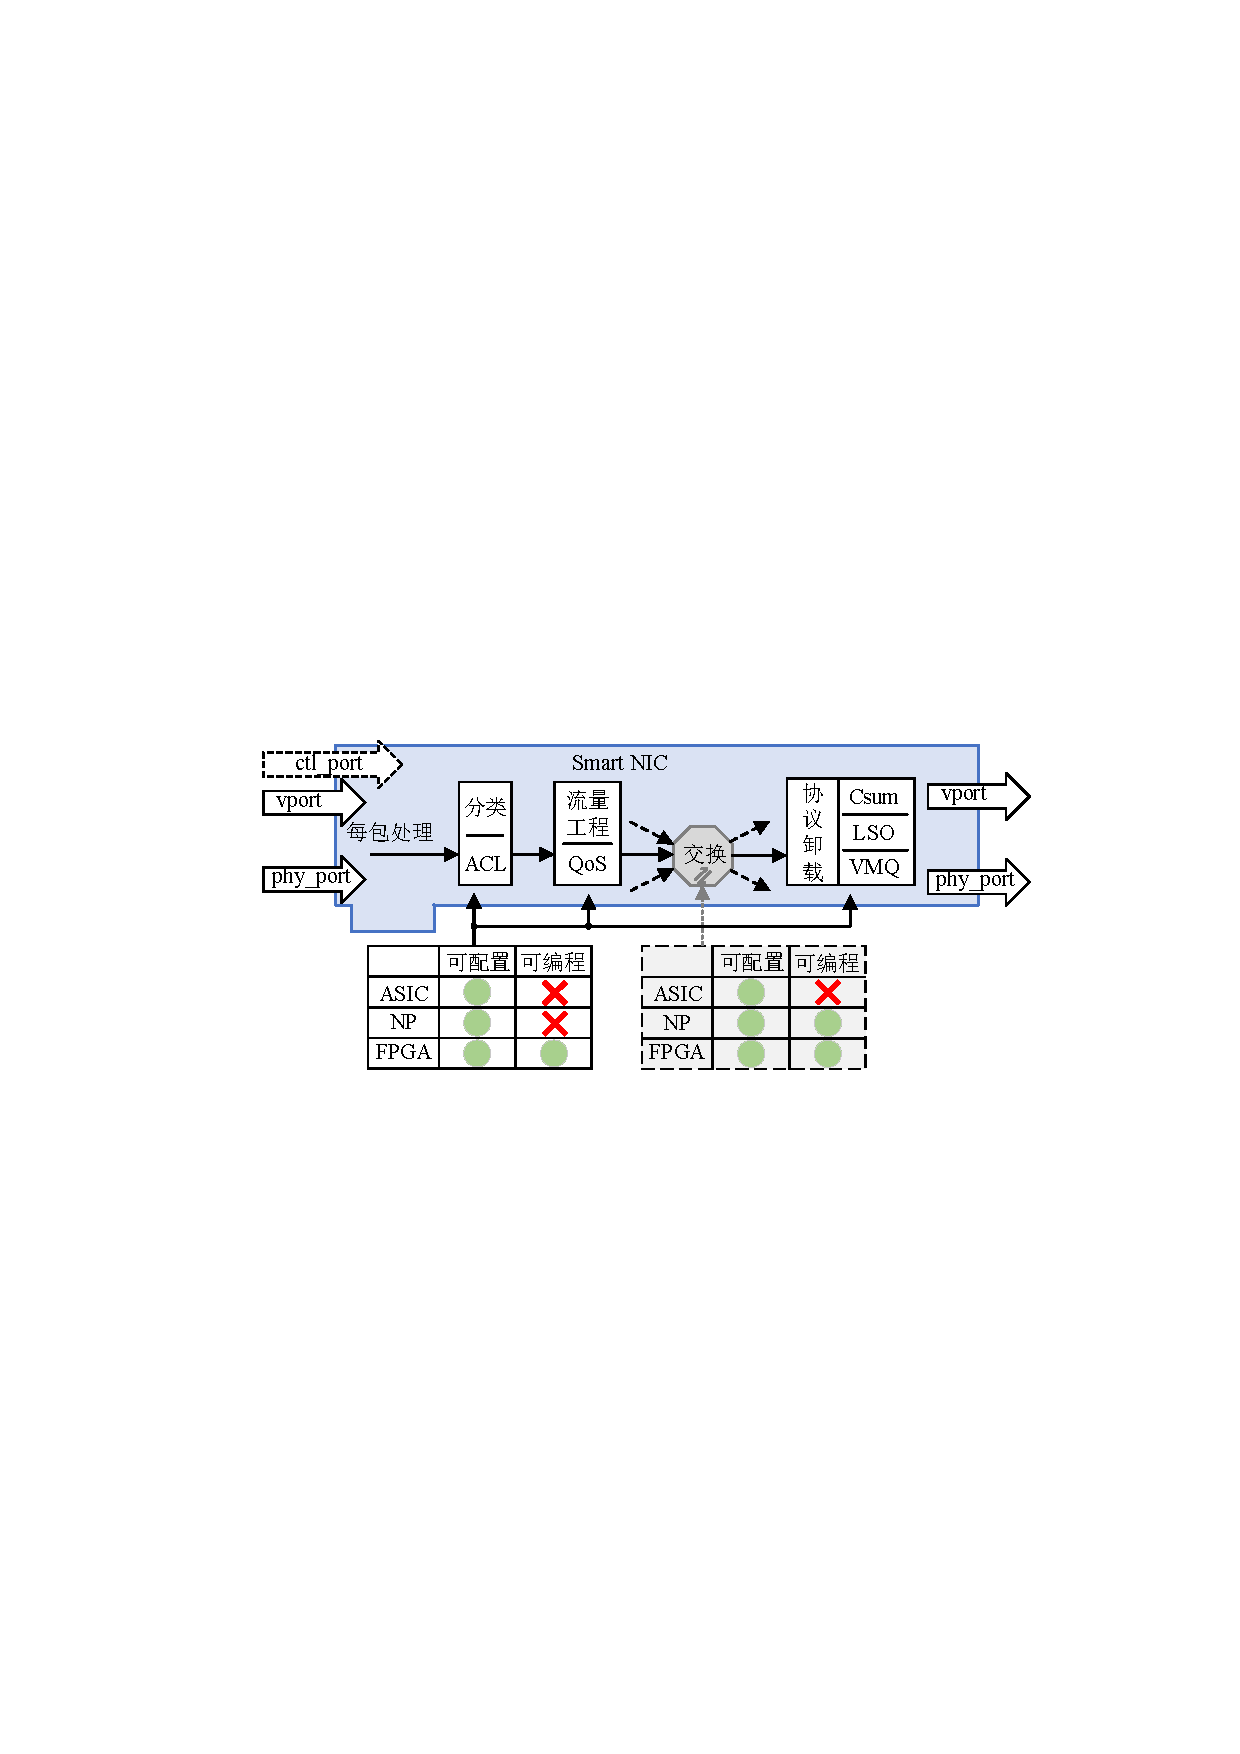
\includegraphics[scale=1]{smartnic.pdf}
%	\caption{各类智能网卡架构及其可编程性对比} \label{fig:smartnic}
%\end{figure}





%1)通用可编程的智能网卡



%\begin{figure}[!ht]
%	\centering 
%	\vspace{-1.5mm}
%	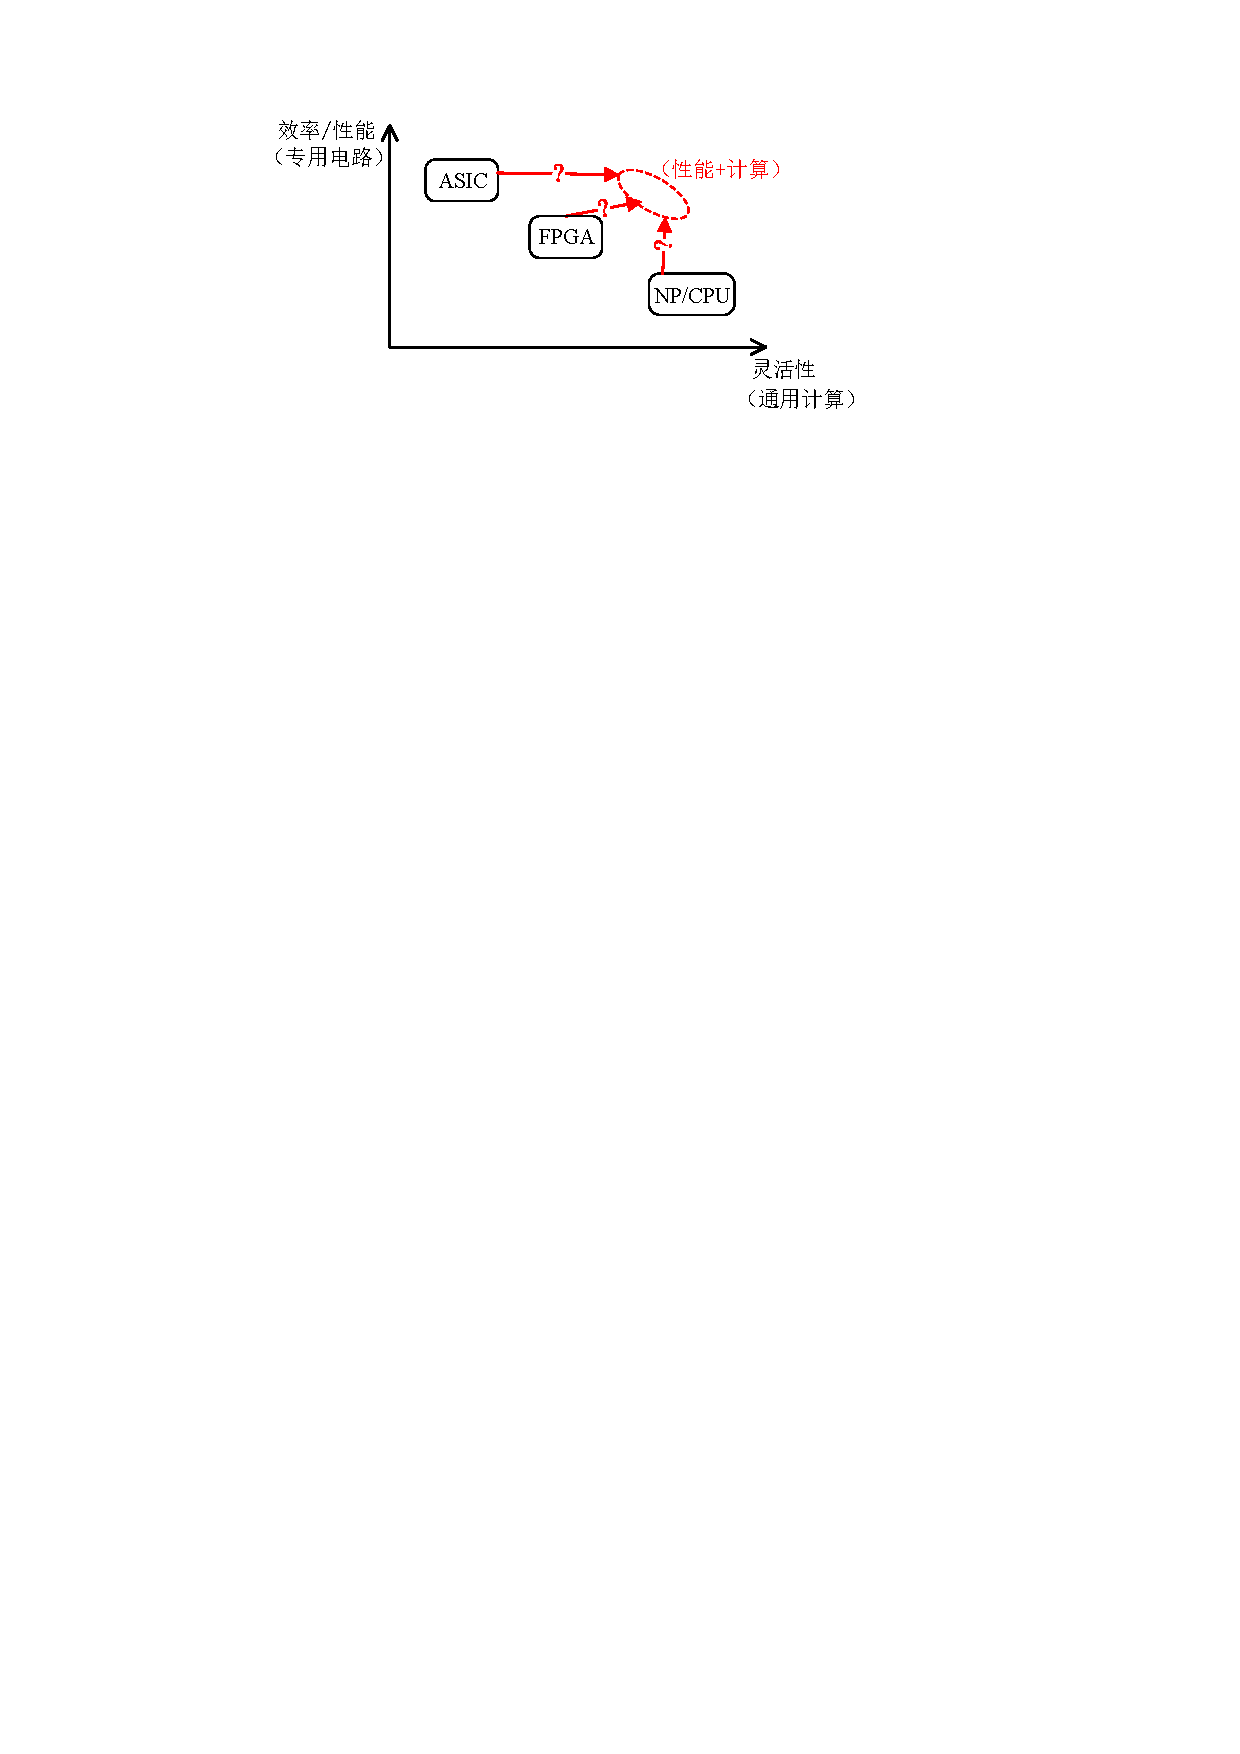
\includegraphics[scale=1]{generalprog.pdf}
%	\caption{性能与灵活性如何更好地折中} \label{fig:generalprog}
%\end{figure}

%2)灵活性与性能
%
%基于目前业界的技术,为设计更灵活的数据平面,我们一般选取如下两种类型的系统做比较:其一,基于NP或CPU众核的智能网卡,拥有比较好的可编程性和灵活性,是具有“图灵完备”一类型设备,我们可以将其当做CPU(计算)系统的延伸。但是他们的缺点也很明显:性能低,效率不足。其二,基于FPGA的智能网卡由于可以任意制定处理逻辑,也属于“图灵完备”的一系列设备。虽然HDL语言是高级描述语言可编程性强,但需要程序员基于硬件电路的思想来完成设计,学习成本高。这种思想层面中的“不灵活”作为一种挑战,又阻碍了FPGA的适用性。性能和可计算性如何更好地折中,或者如何选取一个更合适演进的线路图则成为本文主要考量之处。






\BiSubsection{专用领域系统的编程支持}{Programmable Forwarding Devices and In-Field Programmability}\label{chap232}%ipad笔记本





%网络测量是支持以上功能的主要手段,因此,我们将这些网络功能可编程性概括为,
%
%统计+触发的模型,也就是说,在数据平面的硬件内,对所有流进行统一的测量,
%
%然后上层软件选择感兴趣的计数值,以及触发方式,共同构建起不同的网络功能。同时也提高这些网络功能的性能,和效率。
%
%完成这个工作的难点在于高速缓存资源受限,因为底层逻辑需要对全空间流量完整的记录统计情况,会占用大量的存储资源,
%
%片外资源在极端情况下难以满足性能需求,多级存储使得系统变得复杂,而且性能保持不稳定。
%
%我们的思路是对计数值进行压缩存储。利用对数运算,使线性增加的统计量的边界快速收敛,解决存储资源问题。其中在优化对数计算时,我们在硬件中,采用概率判断的方式简化对数计算。
%
%为了提高计算精度,我们使用分段计数法,前期采用线性统计,流量庞大的流采用压缩统计,使得两部分的统计精度都保持在比较高的水平。
%
%最后我们在基于FPGA的网卡上实现了,一套可编程的网络测量系统,将大部分呆滞重复的软件任务卸载到FPGA 中,在增加吞吐性能的同时,极大的降低了资源消耗。


%1)领域内可编程性



%在不同的信息技术领域内有不同信息处理需求,从信息技术蓬勃发展的过去的几十年到现在,随着微电子行业的诞生,一直不断地涌现出各种类型基于某种专业硬件的处理器,往往这些设备都兼具有某种软件的可编程性。如图\ref{fig:historyprocessors}所示,下面简要介绍历史各个类型可编程处理器。第一,中央处理器(CPU)。CPU解决的是通用类型的计算问题,工作生产生活中,人们往往会遇到各种各样的数学计算任务,使用CPU去辅助人们完成这类枯燥且量大的工作可以极高地提升社会生产效率。CPU采用冯诺依曼结构,是一种图灵机。它将处理通用计算任务抽象为控制-计算-存储模型。控制模块从存储器内读取程序指令和数据指令,并把他们按逻辑分配给计算模块。人们预先可以将需要处理的任务和数据编写到可重复擦写的存储器中,实现各种灵活的任务需求。操作人员就从繁琐的计算当中隔离开来,只需要去关注如何设计控制逻辑已经对应的需要计算的数据。
%\begin{figure}[!ht]
%	\centering 
%	\vspace{-1.5mm}
%	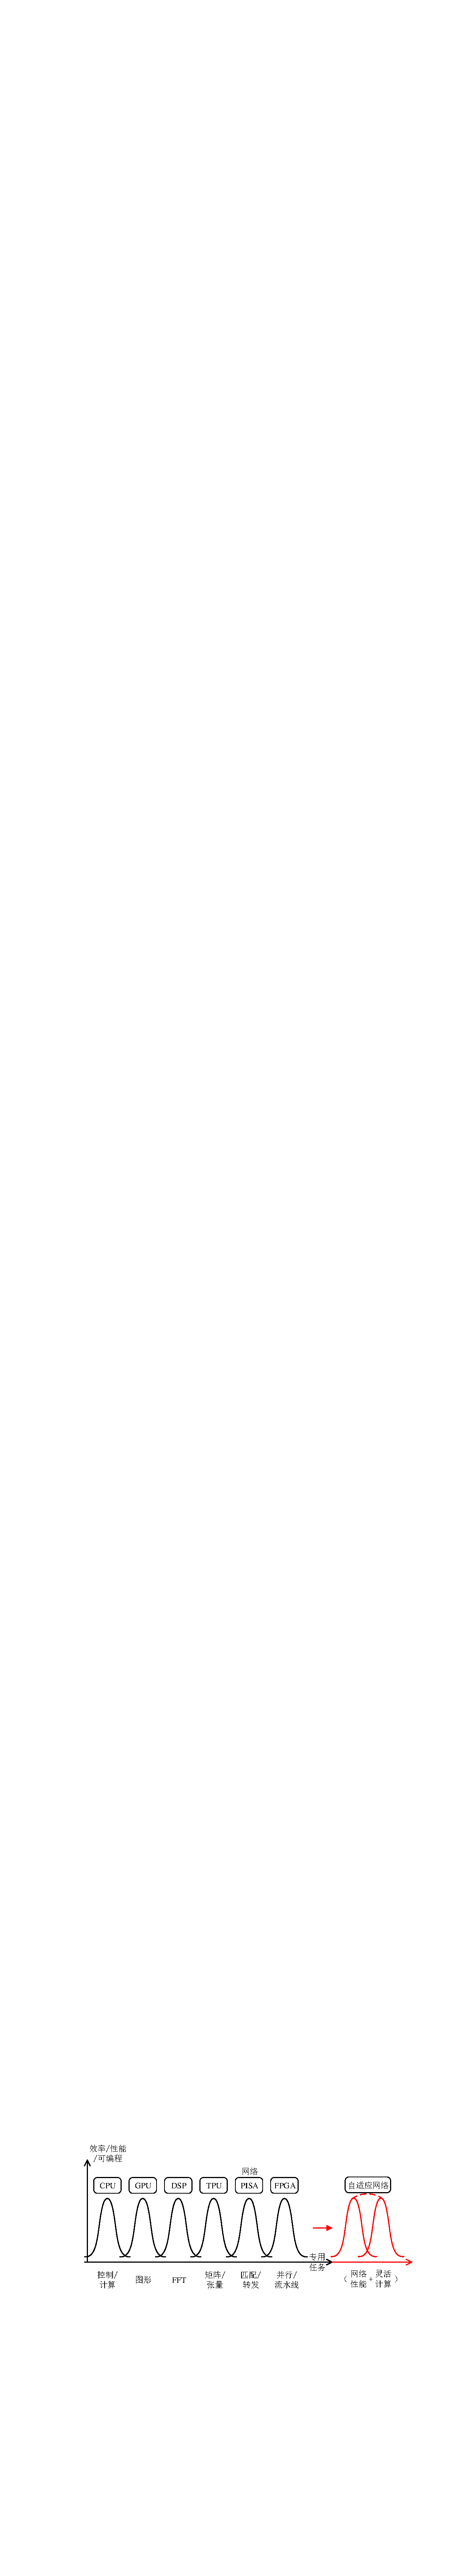
\includegraphics[scale=1]{historyprocessors.pdf}
%	\caption{器件在不同的专用任务中性能和可编程性指标} \label{fig:historyprocessors}
%\end{figure}

%第二,图形处理器(GPU)。图形从本质上是一组二维矩阵数据,像素数据量一般都在百万级别。视频信号又是由一帧一帧的图像先后排列形成,导致处理图形的过程中产生大量的数据量。这些数据由CPU处理往往需要占用很长的处理时间,消耗大量的计算能力从而效率低下。GPU架构提出,图像处理没有先后依赖关系,处理器对于每一帧图像处理的方式完全一致,因而可以利用多CPU并行处理以达到加速目的。所以GPU就是众多微小的CPU的堆叠,同时增加了片上存储密度以应对并发的指令读取需求。第三,信号处理器(DSP)。与CPU类似,但DSP增加了专门为信号处理设计的指令集,使FFT运算更快速。DSP一般是数据地址与内存地址分开的双总线结构,支持灵活的编程。第四,神经网络处理器(NPU)。神经网络的训练过程需要进行大量的张量运算,适合于使用并行度高的处理器做运算,例如使用GPU。但在神经网络的计算中数据位宽往往比较低(8bits),如果使用通用处理器会有比较大的资源浪费,能源效率也比较低。随着AI技术发展,业界对算力的需求持续增高,研究人员专门为神经网络计算任务设计了一种专用处理芯片,TPU与GPU相比在同样能源消耗下,计算完成时间可缩短70倍左右\citeup{tpugoogle}。第五,协议无关交换架构(PISA)。网络包处理流程一般比较封闭,开发人员一般使用设备厂商固化好的网络设备进行数据包传输处理等。但由于网络功能应用环境的快速变化,研究人员发现固化的网络处理芯片无法满足增加新协议的需求,这严重制约了网络的创新。最近业界提出基于硬件的PISA模型,定义了可编程数据包处理的规范。它提出了开源的数据平面功能描述语言,为开发人员提供了可编程的包头描述能力,以及对应的包头信息抽取。在查找和匹配方法上,此类芯片使用多级查表法来实现任意的匹配和查找操作。



%在网络领域的可编程虽然较新,但已经引发业界很大的关注。可编程网络在超大规模数据中心网络、企业级交换网、网络内测量、负载均衡等领域都有广泛的实践以及优势\citeup{miao2017silkroad,li2019hpcc,yang2018elastic}。PISA有能力只使用单一器件就可支持种类繁多的网络功能,这种高的灵活性可为企业节约更换设备的成本,统一结构的数据平台也使操作人员维护复杂网络的成本降低。综上所述,网络可编程已经作为可编程专用任务中的重要一分子,在未来值得持续投入研究。

%0)可编程的介绍
%1)如何引出可编程交换机
%2)详细介绍












%多少MB,电能

%查找表资源占比大。

%TCAM 面积 举例子 金额



\BiSection{本章小结}{Conclusion}\label{chap25}













































